% Ejemplo de documento LaTeX
% Tipo de documento y tamaño de letra
\documentclass[12pt]{article}


\usepackage[spanish]{babel}
\usepackage{longtable} 
\selectlanguage{spanish}
\usepackage[utf8x]{inputenc}
\usepackage{graphicx}




% EL titulo, autor y fecha del documento
\title{Reporte de Actividad 6}
\author{Carlos Medina}
\date{10-04-15}


% Aqui comienza el cuerpo del documento
\begin{document}
% Construye el título
\maketitle


El siguiente reporte describirá los pasos realizados para la actividad 7 (2015-1), se explicarán y se mostrarán los resultados de ésta.




\hspace {0.5cm} En este reporte estudiaremos las mareas, los tipos de mareas, sus comportamientos, y verémos cómo calcular las mareas altas y bajas en un periodo de tiempo como un mes e incluso un día.

\section{¿Cómo se originan?}

El origen de las fuerza de marea se debe a que la Tierra es un cuerpo extenso y el campo gravitatorio producido por la Luna o por el Sol no es homogéneo en todos sus puntos, ya que hay unos puntos que están más cercanos y otros más alejados de dichos cuerpos celestes.

 
\begin{center}
	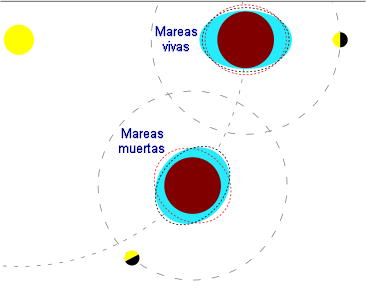
\includegraphics[width=8cm]{mar.png}\\
\end{center}
 
El elipsoide debido a las mareas solares tiene el eje mayor dirigido hacia el Sol. El elipsoide debido a las mareas lunares tiene el eje mayor dirigido hacia la Luna. Como la Luna gira alrededor de la Tierra, los ejes mayores de los elipsoides no giran a la misma velocidad.

	Con respecto a las estrellas, el periodo de rotación del elipsoide solar es de un año. El elipsoide de la Luna es de 27,32 días. El resultado es que los ejes de los dos elipsoides se acercan cada 14,7652944 días.
	
	 Cuando los ejes mayores de los dos elipsoides están alineados, la amplitud de las mareas es máxima y se llaman mareas vivas o mareas sizigias. Esto sucede en las lunas nuevas y en las lunas llenas. En cambio, cuando el eje mayor de cada elipsoide está alineado con el eje menor del otro, la amplitud de las mareas es mínima. Esto sucede en los cuartos menguantes y los cuartos crecientes. Estas mareas se llaman mareas muertas o mareas de cuadratura.
	 
	 
\section{Historia}	 
	 
	 El fenómeno de las mareas es conocido desde la antigüedad. Parece ser que Piteas (siglo IV a. C.) fue el primero en señalar la relación entre la amplitud de la marea y las fases de la Luna, así como su periodicidad. Plinio el Viejo (23-79) en su Naturalis Historia describe correctamente el fenómeno y piensa que la marea está relacionada con la Luna y el Sol. 

 
\begin{center}
	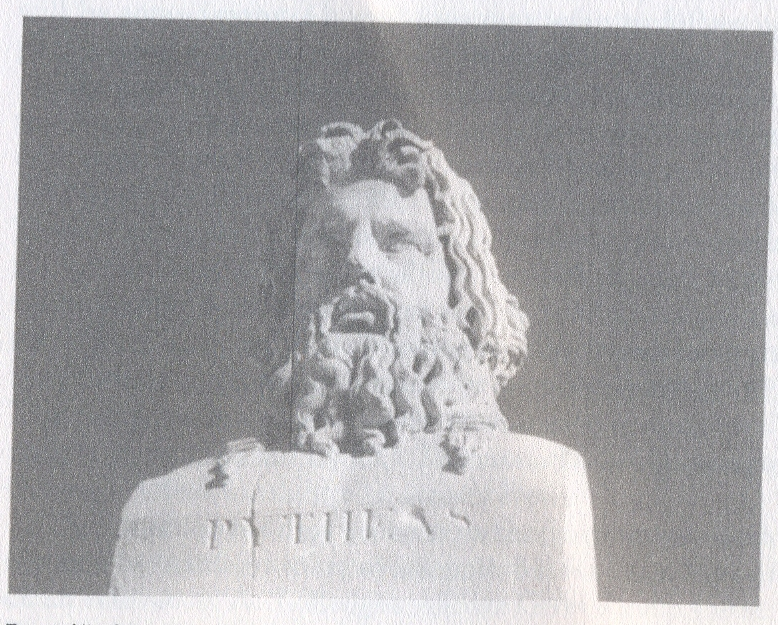
\includegraphics[width=5cm]{piteas.png}\\
\end{center}	 
	 
	 Mucho más tarde, Bacon, Kepler y otros trataron de explicar ese fenómeno, admitiendo la atracción de la Luna y del Sol. Pero fue Isaac Newton en su obra Philosophiae Naturalis Principia Mathematica («Principios matemáticos de la Filosofía Natural», 1687) quien dio la explicación de las mareas aceptada actualmente. Más tarde, Pierre-Simon Laplace (1749-1827) y otros científicos ampliaron el estudio de las mareas desde un punto de vista dinámico.

Isaac Newton realizó varios estudios científicos del comportamiento de las mareas y calculó la altura de éstas según la fecha del mes, la estación del año y la latitud. Más tarde, Simon Laplace complementó los estudios de Newton.
	 
	 \begin{center}
	
\includegraphics[width=8cm]{niuton.jpg}\\
\end{center}	 
	 
\section{Analizando las mareas}

	Ahora, analizaremos un ejemplo de mareas reales con un archivo con datos que nos ha proporcionado el Dr. Julio César Rodríguez, del Departamento de Agricultura. Los datos se proporcionan en un archivo en formato de Excel, que puedes descargar de aquí. Los datos corresponden al manglar El Sargento, ubicado en la costa, cerca del Desemboque de los Seris, casi frente a la Isla del Tiburón.
	
		 \begin{center}
	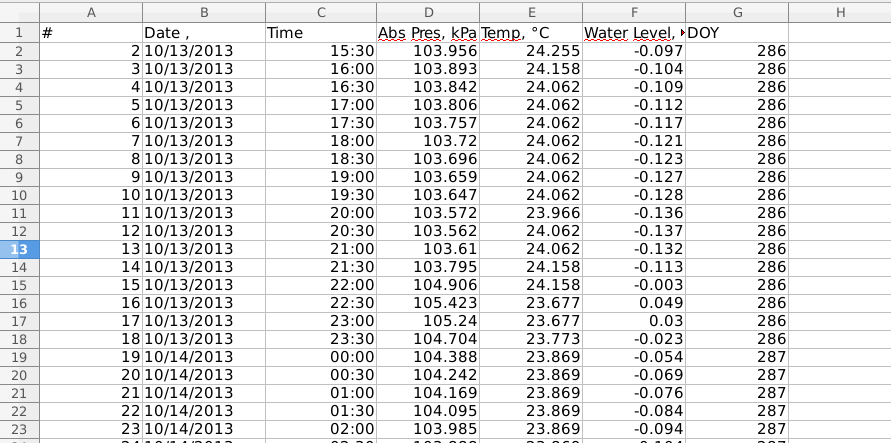
\includegraphics[width=10cm]{d.png}\\
\end{center}	 
	
	Primeramente, procedemos a procesar los datos de una forma que fortran los pueda leer.
	
		 \begin{center}
	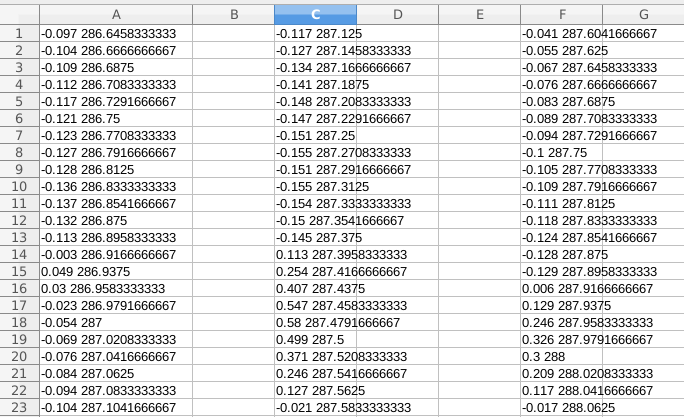
\includegraphics[width=10cm]{d2.png}\\
\end{center}	 

Ahora, proseguimos con iniciar el código de fortran para que calcule las alturas máximas y mínimas en los primeros 5 meses y los primeros 5 días.

\begin{verbatim}
program Mareas

implicit none
real, dimension (7674):: Altura
integer :: i
real :: perro, Maxd1, Maxd2, Maxd3, Maxd4, Maxd5 
real :: Max1, Max2, Max3, Max4, Max5
real :: gato, Mind1, Mind2, Mind3, Mind4, Mind5 
real :: Min1, Min2, Min3, Min4, Min5
real :: Tiempo11, Tiempo21, Tiempo31, Tiempo41, Tiempo51
real :: Tiempo12, Tiempo22, Tiempo32, Tiempo42, Tiempo52
real :: Dif1, Dif2, Dif3, Dif4, Difm1, Difm2, Difm3, Difm4, T1, T2, T3, T4, T5, T1m, T2m, T3m, T4m, T5m

open (1,file="Mareas.csv")

do i=1,7674
read (1,*) Altura(i)
end do
close (1)

!---------------------------------------------------------------------------------------------------------------------------------------------------------------
!Maximas y minimas del primer mes (Valores del 1 al 1344)

Max1 = 0
do i=1,1344
perro = Max1-Altura(i)
if (perro<0) then 
Max1 = Altura(i)

Tiempo11=i/48.0
end if
end do



Min1 = 0
do i=1,1344
gato = Min1-Altura(i)
if (gato>0) then
Min1 = Altura(i)

Tiempo12=i/48.0
end if
end do


!-------------------------------------------------------------------------------
!Maximas y minimas del segundo mes 

Max2=0
do i=1345,2689
perro= Max2-Altura(i)
if (perro<0) then 
Max2 = Altura(i)

Tiempo21=i/48.0
end if
end do

Min2 = 0
do i=1345,2689
gato = Min2-Altura(i)
if (gato>0) then
Min2 = Altura(i)

Tiempo22=i/48.0
end if
end do


!-------------------------------------------------------------------------------
!Maximas y minimas del tercer mes

Max3=0
do i=2690,4034
perro= Max3-Altura(i)
if (perro<0) then 
Max3 = Altura(i)

Tiempo31=i/48.0
end if
end do

Min3 = 0
do i=2690,4034
gato = Min3-Altura(i)
if (gato>0) then
Min3 = Altura(i)

Tiempo32=i/48.0
end if
end do


!-------------------------------------------------------------------------------
!Maximas y minimas del cuarto mes

Max4=0
do i=4035,5379
perro= Max4-Altura(i)
if (perro<0) then 
Max4 = Altura(i)

Tiempo41=i/48.0
end if
end do

Min4 = 0
do i=4035,5379
gato = Min4-Altura(i)
if (gato>0) then
Min4 = Altura(i)

Tiempo42=i/48.0
end if
end do


!-------------------------------------------------------------------------------
!Maximas y minimas del quinto mes

Max5=0
do i=5380,6724
perro= Max5-Altura(i)
if (perro<0) then 
Max5 = Altura(i)

Tiempo51=i/48.0
end if
end do

Min5 = 0
do i=5380,6724
gato = Min5-Altura(i)
if (gato>0) then
Min5 = Altura(i)

Tiempo52=i/48.0
end if
end do

!---------------------------------------------------------------------------------------------------------------------------------------------------------------
!Maximas y minimas de cada dia
!---------------------------------------------------------------------------------------------------------------------------------------------------------------


Maxd1 = 0
do i=1,48
perro = Maxd1-Altura(i)
if (perro<0) then 
Maxd1 = Altura(i)

T1 = i/2
end if
end do

Mind1 = 0
do i=1,48
gato = Mind1-Altura(i)
if (gato>0) then
Mind1 = Altura(i)

T1m =i/2
end if
end do


!-------------------------------------------------------------------------------


Maxd2=0
do i=49,97
perro= Maxd2-Altura(i)
if (perro<0) then 
Maxd2 = Altura(i)

T2=i/2
end if
end do

Mind2 = 0
do i=49,97
gato = Mind2-Altura(i)
if (gato>0) then
Mind2 = Altura(i)

T2m =i/2
end if
end do


!-------------------------------------------------------------------------------

Maxd3=0
do i=98,146
perro= Maxd3-Altura(i)
if (perro<0) then 
Maxd3 = Altura(i)

T3 = i/2
end if
end do

Mind3 = 0
do i=98,146
gato = Mind3-Altura(i)
if (gato>0) then
Mind3 = Altura(i)

T3m = i/2
end if
end do

!-------------------------------------------------------------------------------

Maxd4=0
do i=147,195
perro= Maxd4-Altura(i)
if (perro<0) then 
Maxd4 = Altura(i)

T4= i/2
end if
end do

Mind4 = 0
do i=147,195
gato = Mind4-Altura(i)
if (gato>0) then
Mind4 = Altura(i)

T4m=i/2
end if
end do

!-------------------------------------------------------------------------------

Maxd5=0
do i=196,244
perro= Maxd5-Altura(i)
if (perro<0) then 
Maxd5 = Altura(i)

T5 = i/2
end if
end do

Mind5 = 0
do i=196,244
gato = Mind5-Altura(i)
if (gato>0) then
Mind5 = Altura(i)

T5m = i/2
end if
end do

!-------------------------------------------------------------------------------

Dif1 = T2-T1
Difm1 = T2m-T1m
Dif2 = T3-T2
Difm2 = T3m-T2m
Dif3 = T4-T3
Difm3 = T4m-T3m
Dif4 = T5-T4
Difm4 = T5m-T4m

Print *, '================°================°====================°================°'
Print *, 'ALTURAS MAXIMAS DE LAS MAREAS:'
Print *, '================°================°====================°================°'
Print *, 'Primer dia:', Maxd1,    'Tiempo para la siguiente maxima:', Dif1
Print *, 'Segundo dia:', Maxd2,   'Tiempo para la siguiente maxima:', Dif2
Print *, 'Tercer dia:', Maxd3,    'Tiempo para la siguiente maxima:', Dif3
Print *, 'Cuarto dia:', Maxd4,    'Tiempo para la siguiente maxima:', Dif4
Print *, 'Quinto dia:', Maxd5    
Print *, '========================================================================'
Print *, 'Primer mes:', Max1, 'En el dia:', Tiempo11
Print *, '---------------------------------------------------------'
Print *, 'Segundo mes:', Max2,'En el dia:', Tiempo21
Print *, '---------------------------------------------------------'
Print *, 'Tercer mes:', Max3,'En el dia:', Tiempo31
Print *, '---------------------------------------------------------'
Print *, 'Cuarto mes:', Max4,'En el dia:', Tiempo41
Print *, '---------------------------------------------------------'
Print *, 'Quinto mes:', Max5,'En el dia:', Tiempo51
Print *, '================°================°====================°================°'
Print *, 'ALTURAS MINIMAS DE LAS MAREAS:'
Print *, '================°================°====================°================°'
Print *, 'Primer dia:', Mind1,    'Tiempo para la siguiente minima:', Difm1
Print *, 'Segundo dia:', Mind2,   'Tiempo para la siguiente minima:', Difm2
Print *, 'Tercer dia:', Mind3,   'Tiempo para la siguiente minima:', Difm3
Print *, 'Cuarto dia:', Mind4,    'Tiempo para la siguiente minima:', Difm4
Print *, 'Quinto dia:', Mind5
Print *, '========================================================================'
Print *, 'Primer mes:', Min1, 'En el dia:', Tiempo12
Print *, '---------------------------------------------------------'
Print *, 'Segundo mes:', Min2,'En el dia:', Tiempo22
Print *, '---------------------------------------------------------'
Print *, 'Tercer mes:', Min3,'En el dia:', Tiempo32
Print *, '---------------------------------------------------------'
Print *, 'Cuarto mes:', Min4,'En el dia:', Tiempo42
Print *, '---------------------------------------------------------'
Print *, 'Quinto mes:', Min5,'En el dia:', Tiempo52
Print *, '================°================°====================°================°'

end program Mareas
\end{verbatim}

Este código, utiliza el "do" para calcular el valor máximo por cada intérvalo de datos, como se ve en el primer mes, es desde el dato 1 al 1344, porque es el número de datos que conforman un mes (ya que un dato es media hora). En esta orden, se establece una operación que llamamos "perro" (por simple humor), y perro es la diferencia entre el valor máximo e "i", después dice "if (perro<0) then valor = Altura(i)" lo que hace que el nuevo Máximo se vuelva "i", y se repite el proceso en los demás meses. Para calcular las alturas máximas de cada día es igual pero con un intérvalo de 48 datos.

Y nos aparece la siguiente pantalla cuando ejecutamos el programa:


\begin{center}
	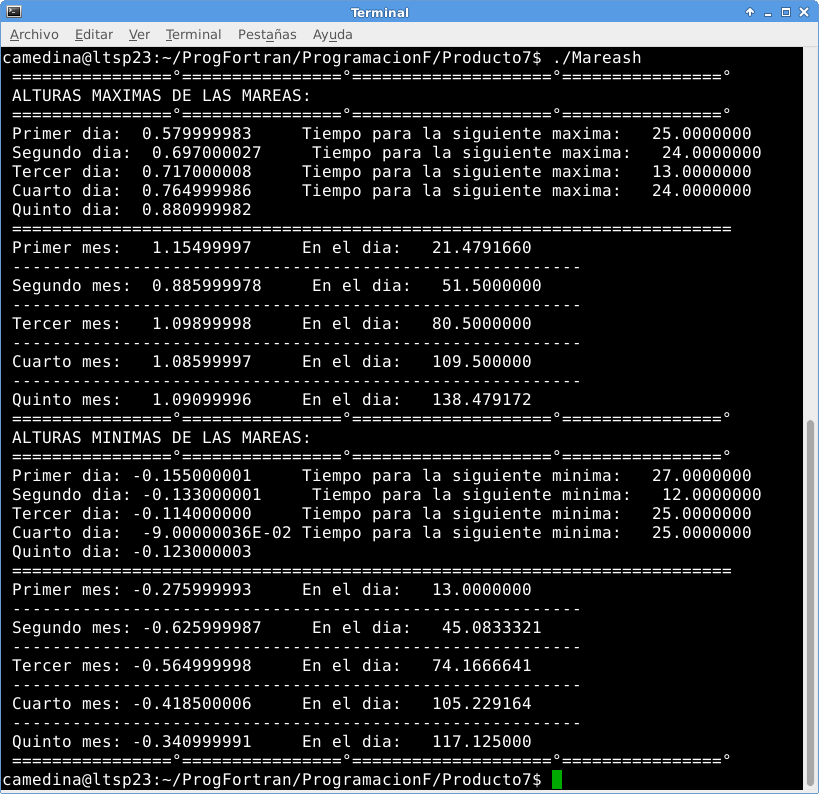
\includegraphics[width=15cm]{prog.png}\\
\end{center}	 

Ahora, procedemos a graficar. La siguiente gráfica es de los primeros tres meses:

\begin{center}
	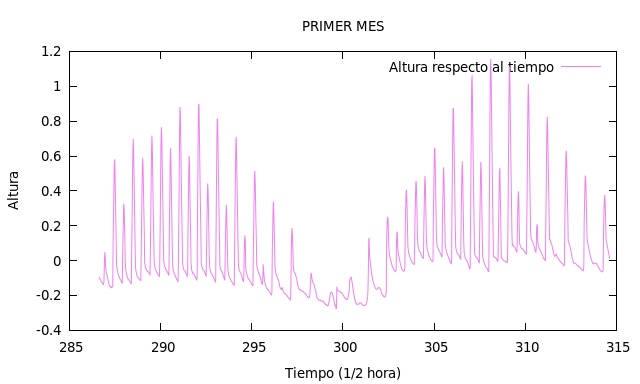
\includegraphics[width=15cm]{graf1m.png}\\
\end{center}	

\begin{center}
	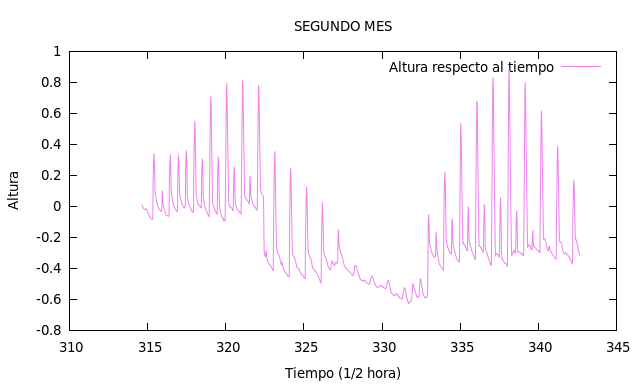
\includegraphics[width=15cm]{graf2m.png}\\
\end{center}	

\begin{center}
	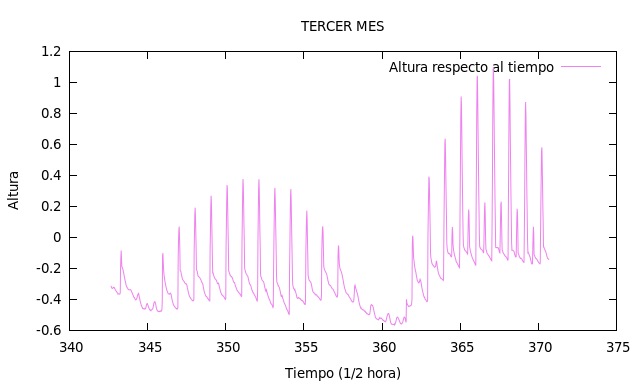
\includegraphics[width=15cm]{graf3m.png}\\
\end{center}	

Ahora, graficar los primeros tres días:


\begin{center}
	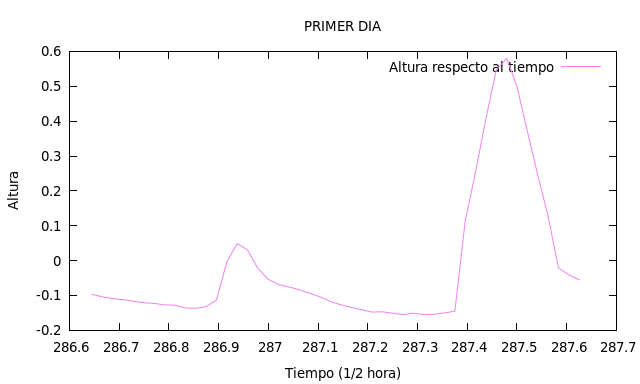
\includegraphics[width=14cm]{graf1d.png}\\
\end{center}	

\begin{center}
	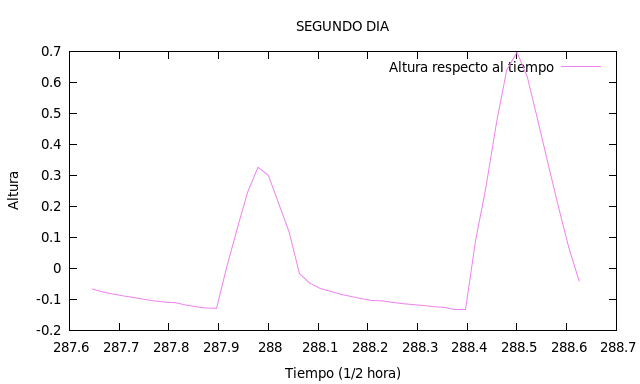
\includegraphics[width=14cm]{graf2d.png}\\
\end{center}	

\begin{center}
	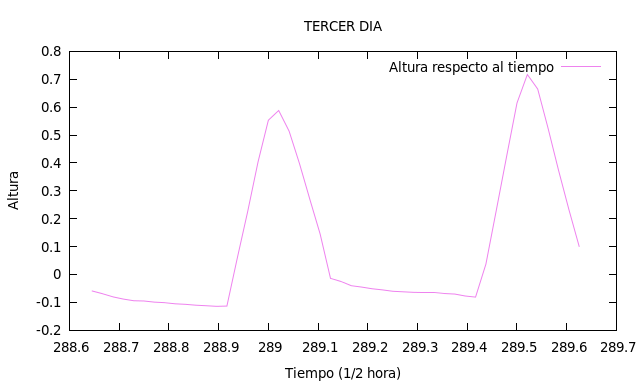
\includegraphics[width=14cm]{graf3d.png}\\
\end{center}	

\section{Conclusión}

	Como conclusión, podemos observar que el periodo de cada marea máxima (pleamar) es de 21.5 horas en promedio, mientras que el periodo para cada marea de mínima altura (bajamar) es de 22.25 horas en promedio.

\end{document}
